% ------------------------------------------------
% Nomenclature list - update if needed
\nomenclature[G]{PoS}{Part of Speech}
\nomenclature[G]{$\mathcal{A}$}{A set of aspect categories for the (T)ABSA tasks}

% ------------------------------------------------

\chapter{Methodology} \label{chapter:methodology}
In this section, we outline our specific methodology for our experiments and define the problem more fully and technically, in line with the project aims outlined in Section \ref{section:intro:projectaims}.

\section{Hypothesis}
We hypothesise that models benefitting from shared related task representations will form better word embeddings for each of the downstream tasks. This is the notion of multitask learning; simultaneously solving many downstream tasks in order to improve performance on each individual task.

We further posit that performance can be improved by looking at \textit{dependent subtasks structures}, and propose to investigate how various task sampling schemas (cf. Definition \ref{def:methodology:taskdistributions}) of these dependent subtasks improves performance on the main task. In our case, the main task we are focusing on is the (T)ABSA tasks - SemEval and Sentihood - explained in Sections \ref{section:background:semeval} and \ref{section:background:sentihood} respectively. We utilise the transformation method described in Section \ref{section:background:tabsasentenceconstruction} to pass this through a language model. Jointly, we will train related subtasks and see how it affects performance.

\section{Task Setup}

\subsection{Task Structure} \label{section:methodology:taskstructure}
In order to solve the TABSA task, we would require performing an ABSA task on each target term individually, so its safe to assume that these tasks are of near equal importance. In order to solve the ABSA task, we would want a language modelling system to be proficient at the following (sub)tasks:
\begin{itemize}
	\item Understanding of sentiment $\rightarrow$ \textbf{Sentiment Analysis Task}
	\item Understanding of aspects $\rightarrow$ \textbf{Part of Speech (PoS)/Named Entity Recognition (NER) Task} from which our model can learn important coreferencing and word disambiguation knowledge from. This is also inspired from the previous SOTA, feature crafted NLP model \cite{Kiritchenko2014} which used PoS and NER features in an SVM model.
\end{itemize}
Due to the way we have set up the (T)ABSA tasks, as per Section \ref{section:background:tabsasentenceconstruction}, one could argue that the model should consider a QA or NLI subtask from which to learn. However, the authors of the auxilliary sentence augmentation technique hypothesise that the reason the BERT pretrained LM is capable of performing so well under this construction is due to the NLI next sentence prediction task during training \cite{Sun2019}. This conjecture was largely unsubstantiated or tested in the paper. We thus propose not to include such a task, but a discussion of this is deferred to Section \ref{section:extensions:subtasks}.

We want to formalise this notion of ``supporting subtasks" that we use in this thesis, and we do so mathematically in the Section \ref{section:methodology:taskdistributions}. Then, in Section \ref{section:methodology:modelsetup}, we describe how we use these notions to complete a forward pass of the multitask model. In the next section, we will discuss the datasets we use motivated by the above analysis.

\subsection{Datasets} \label{section:methodology:datasets}
As is common in the NLP literature, we refer to ``labels" as the target classes, and our models are performing multiclass classification.
\begin{center}
	\resizebox{\textwidth}{!}{%
		\begin{tabular}{c@{\qquad}cccc@{\qquad}|ccc}
			\toprule
			\multirow{2}{*}{\raisebox{-\heavyrulewidth}{Tasks (Datasets)}} & \multicolumn{4}{c}{Properties} & \multicolumn{3}{c}{Size} \\
			\cmidrule{2-8}
			& Priority & \# Labels & \# Sentiment Classes & \# Aspects & Train & Dev & Test\\
			\midrule
			TABSA$^\dagger$ (Sentihood) & Primary & 2 & 3 & 4  & 2952 & \multicolumn{2}{c}{872} \\
			ABSA$^\dagger$ (SemEval 2014)\footnotemark & Primary & 2 & 5 & 5  & 3038 & \multicolumn{2}{c}{747} \\
			Sentiment Analysis (SST-2)\footnotemark & Secondary & 2 & 2 & - & 67349 & \multicolumn{2}{c}{872} \\
			PoS (CoNLL 2003) & Secondary & 45 & - & - & 14041 & 3250 & 3453 \\
			\hline
			Sentiment Analysis (IMDB)$^*$ & Secondary & 2 & 2 & - & 19872 & 9975 & 19872 \\
			\hline
			Classification$^\dagger$ (Streetbees Data) & Primary & 2 & - & 34 & 24303 & \multicolumn{2}{c}{3097} \\
			\bottomrule
	\end{tabular}}
	\captionof{table}{Datasets used throughout this thesis, including various properties of each dataset. $^*$ denotes dataset only used for preliminary testing (cf. Section \ref{section:experiments:sentimentonly}) \newline $^\dagger$ denotes using the QA\_\textbf{B} method to create the exploded dataset as described in Table \ref{table:background:tabsasentencesB}. All sizes are given prior to the explosion of the dataset i.e the raw number of input text sentences for each dataset. In some cases, the dev set is equal to the test set, to match the reporting statistics given in various papers and since we are fixing hyperparameters as per \cite{Sun2019} so no hyperparameter tuning is required}
	\label{table:methodology:datasets}
\end{center}
\addtocounter{footnote}{-2} %We made 2 footnote marks in the table so subtract it manually and add as below
\stepcounter{footnote} \footnotetext{specifically Task 4, Subtask 4, Restaurants dataset}
\stepcounter{footnote} \footnotetext{There is an unlabelled test set of $\sim$1k datapoints, but since reporting is often done on the dev set and is so for the papers to which we are comparing to, we keep the splits despite the heavy skew in training and dev/testing sets}

Table \ref{table:methodology:datasets} shows the datasets we employ for testing. We decided to focus on the QA\_\textbf{B} ``explosion" method for several reasons:
\begin{enumerate}
	\item It was SOTA across the board for the SemEval (ABSA) task and achieved the largest $F_1$ score on aspects and AUC on Sentiment for the Sentihood (TABSA) task
	\item The Streetbees data was actually a multi-aspect classification problem, and so we needed to have a probability for each of the aspects so we could map this onto a multi aspect output.
	\item The BERT pretraining NLI objective was itself binary - it was next sentence prediction. We hypothesised that this would enable the best performance for BERT
\end{enumerate}

\subsubsection{(T)ABSA Data}
The reader is deferred to the discussion in Sections \ref{section:background:semeval}, \ref{section:background:sentihood} and \ref{section:background:tabsasentenceconstruction} for how this data was prepared, as it is equivalent to the methods utilised in the Auxilliary Construction Method paper \cite{Sun2019}. As mentioned, we focused on the QA\_\textbf{B} method for this thesis.

\subsubsection{SST-2}
The reader is deferred to Section \ref{section:background:sst2} for a more in depth discussion of this dataset. We use the standard dataset downloaded from the GLUE benchmark tasks \cite{Wang2018}.

\subsubsection{PoS}
For the PoS task, we focus on the CoNLL 2003 Dataset \cite{Tjong} which has become the benchmark for PoS and NER testing. The authors released both an English and German version, on which we focus on the English version. As is common in NLP, we refer to the corresponding ``label" which comes from a set of classes, so the goal for this dataset is multiclass classification. The dataset is best illustrated via an example:

\begin{center}
	\begin{tabular}{||c | c | c | c||} 
		\hline
		Token & PoS Label\footnotemark & Chunking Label & NER Label  \\ [0.5ex] 
		\hline\hline
		U.N. & NNP & I-NP & I-ORG\\
		official & NN & I-NP & O\\
		Ekeus & NNP & I-NP & I-PER\\
		heads & VBZ & I-VP & O\\
		for & IN & I-PP & O\\
		Baghdad & NNP & I-NP & I-LOC\\
		. & . & O & O\\
		\hline
	\end{tabular}
	\captionof{table}{An example of the tagging schemas for CoNLL 2003}
	\label{table:methodology:nerexample}
\end{center}
\footnotetext{A comprehensive list of what these labels mean can be found at \href{{https://www.ling.upenn.edu/courses/Fall_2003/ling001/penn_treebank_pos.html}}{\texttt{https://www.ling.upenn.edu/courses/Fall\_2003/ling001/penn\_treebank\_pos.html}}. However, the reader should just be aware that these symbols roughly correspond to whether or not the word is a noun, adjective, pronoun, verb etc.}

We choose to focus on the PoS task for our use case. The NER task focuses on entities such as people, locations and organisations. Since our ABSA task requires the model to understand how adjectives are related to nouns, and its only the TABSA task that really requires notions of locations (which are themselves proper nouns) we decided that it was more relevant for the model to work on a PoS task simultaneously as it would generalise better in both the ABSA and TABSA settings.


\subsubsection{Streetbees Data} \label{section:data:streetbees}
We also take the opportunity in this thesis to apply these methods on corporate data. More information about the company partnered with this thesis, and the type of work they do, can be found in Appendix \ref{appendix:streetbees}. As a brief introduction, the company conducts consumer behaviour surveys. The goal for this particular dataset was to ascertain how individuals felt emotionally when buying a product. An ontology was constructed, resulting in numerous categories. This was a multilabelled problem, since it was possible that users could be feeling several emotions simultaneously.

To improve the quality of the labels, we filter the data so that only the labels with at least 100 unique datapoints are included, thus avoiding labels with very sparse support. Figure \ref{fig:methodology:streetbeesdatahist} shows a count of unique datapoints with corresponding label categories.
\begin{center}
	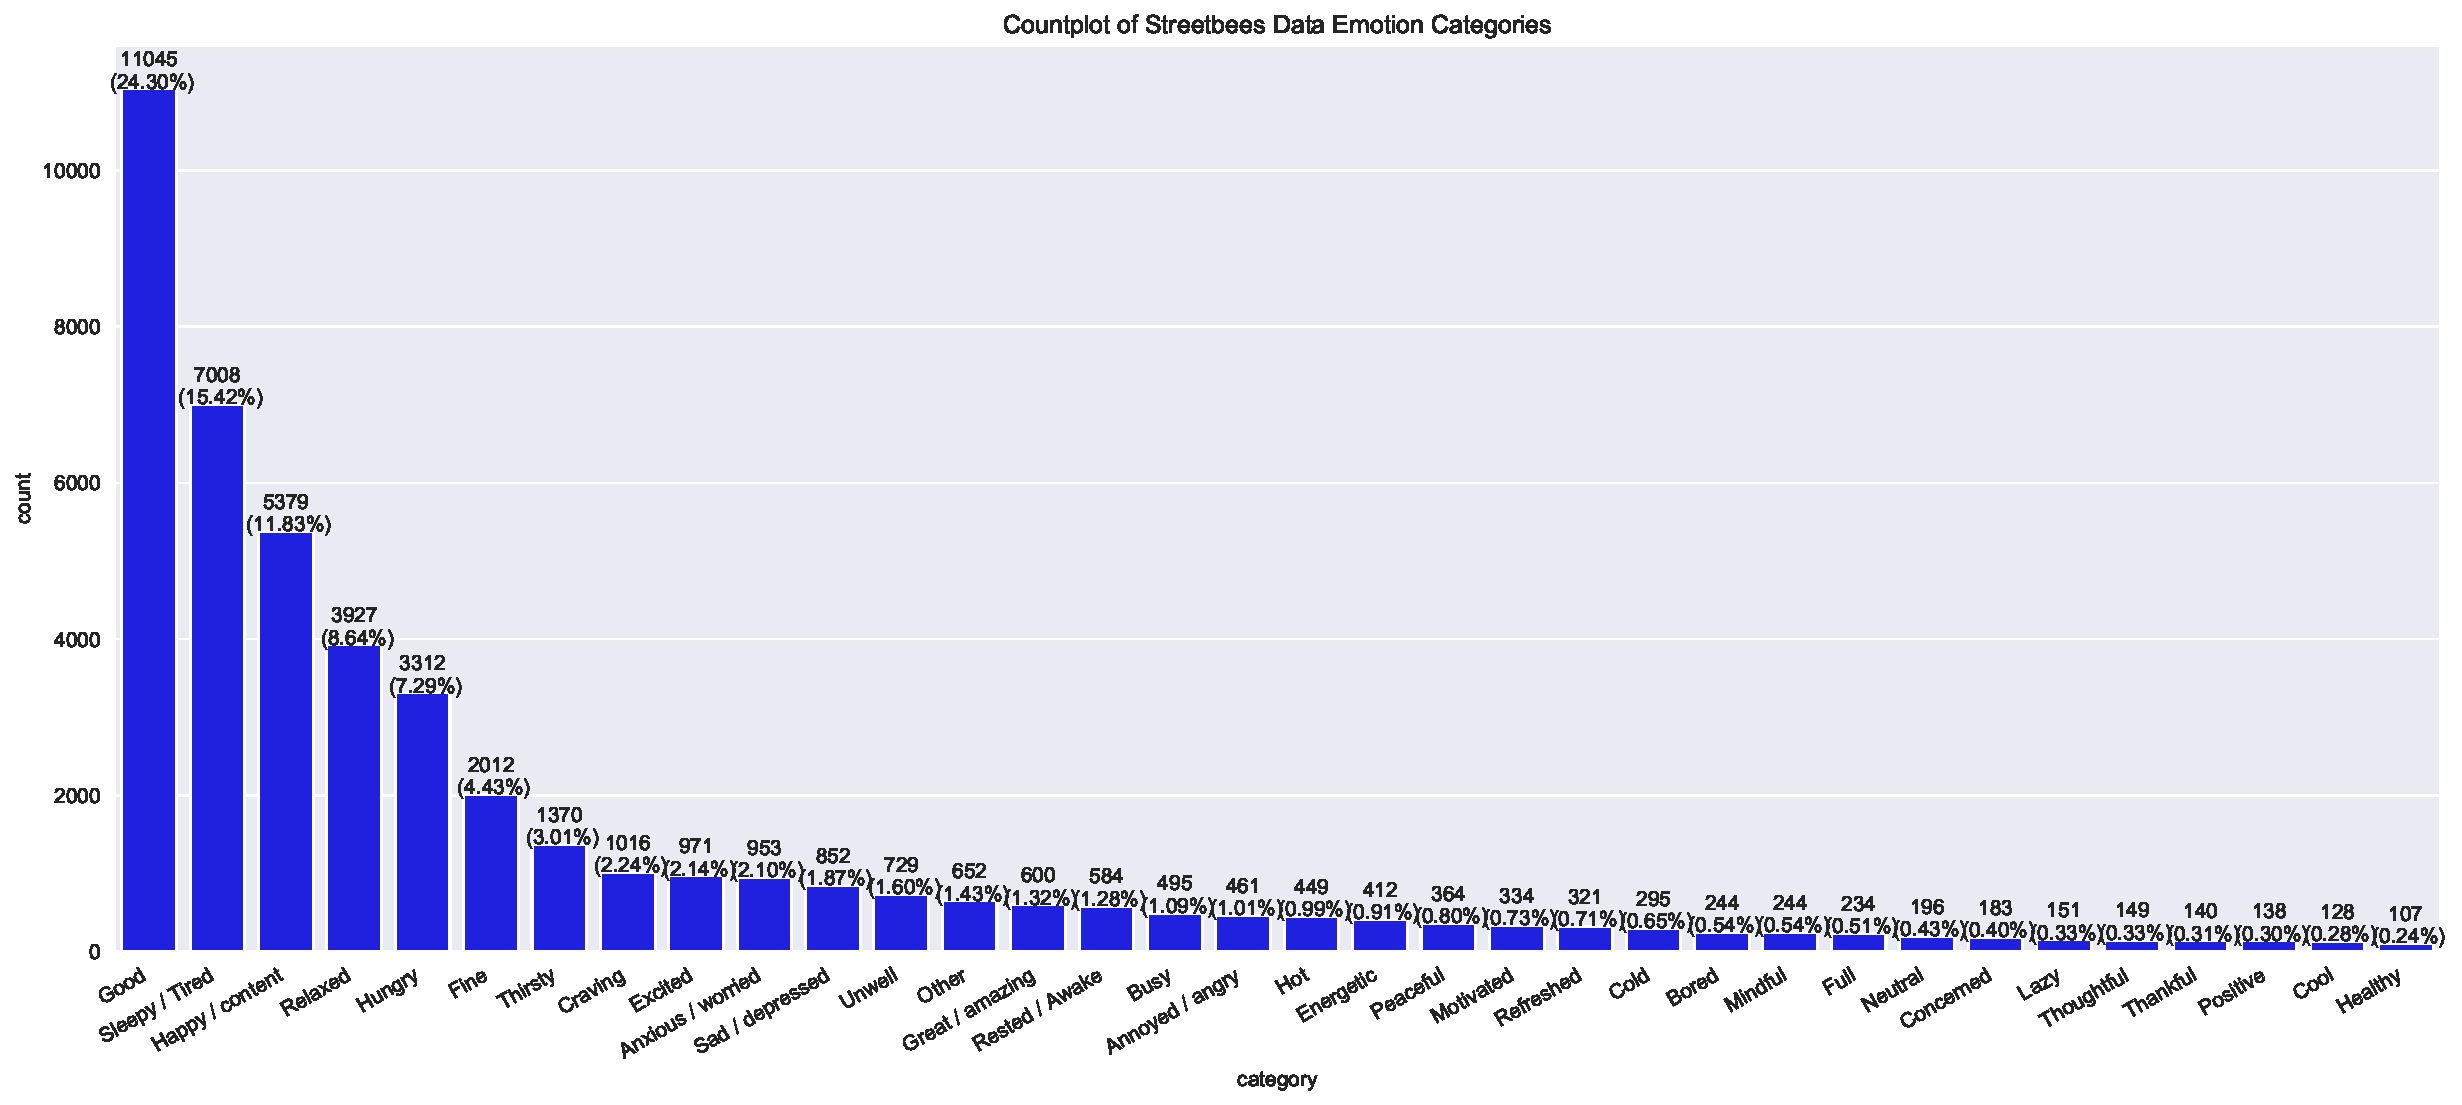
\includegraphics[width=\textwidth]{streetbees_data_hist.pdf}
	\captionof{figure}{Countplot of the Streetbees Data (emotion) categories}
	\label{fig:methodology:streetbeesdatahist}
\end{center}

We prepare the data in the QA\_\textbf{B} format as per Table \ref{table:background:tabsasentencesB}, with the prepending question string \texttt{`Do you feel'} i.e we ask questions \texttt{Do you feel} $e$ \texttt{?} for emotion $e \in \mathcal{C}$ and have binary labels. Due to the sheer number of classes, we avoid the sparsity problem of the exploded dataset by including all the positive examples as well as 5 negative class samples. This enables the model to learn much better when the number of classes is large, and is in line with the ABSA explosion method in terms of the number of aspects per datapoint.

The core advantage of this binary explosion method is that it gives probability scores of each of the emotion categories, enabling us to select multi labelled output when the probability of an emotion exceeds a certain probability threshold, which we set to the natural value of 0.5.

\subsection{Task Distributions} \label{section:methodology:taskdistributions}
We begin by defining some important concepts that will be used throughout. A task is synonymous with a dataset, as per Table \ref{table:methodology:datasets}.
\begin{definition}[Sampling Distributions] \label{def:methodology:samplingdistributions}
	A sampling distribution is the probability distribution of the sample statistic. For our purposes, the sample statistic will be a single task drawn from a categorical distribution i.e get $\tau_i \in \mathcal{T} = \{\tau_1, \dots, \tau_n\}$ with $\P(t = \tau_i | \mathbf{p}, e) = p_{\tau_i}$, where $\mathbf{p} = \begin{pmatrix} p_{\tau_1}, \dots, p_{\tau_n} \end{pmatrix}$ and $e$ is our current epoch (cf. the annealing strategy in Definition \ref{def:methodology:taskdistributions}). 
	
	In an abuse of terminology, we will refer to the sequential progression through tasks (i.e $\tau_1 \rightarrow \tau_2 \rightarrow \dots \rightarrow \tau_n \rightarrow \tau_1 \rightarrow \dots$) as a sampling distribution, despite its determinism.
\end{definition}
\begin{definition}[Task Weighting] \label{def:methodology:taskweightings}
	Define the weight of a task $\tau_i$ to be $w_{\tau_i} \in \mathbb{R}$.
\end{definition}
\begin{definition}[Task Distribution] \label{def:methodology:taskdistributions}
	The task distribution is our sampling distribution over tasks. With the same notation as in Definition \ref{def:methodology:samplingdistributions}, we in general define $p_{\tau_i} = \frac{w_{\tau_i}^{\alpha_s (e)}}{\sum \limits_{k=1}^{n} w_{\tau_k}^{\alpha_s (e)}}$ for strategy $s$. The strategies we are considering are:
	\begin{enumerate}
		\item \textbf{Random:} $\alpha = 0 \Rightarrow p_{\tau_i} = \frac{1}{n}$ i.e uniformily at random sampling tasks from $\mathcal{T}$.
		\item \textbf{Prop(ortional):} $\alpha = 1 \Rightarrow p_{\tau_i} = \frac{w_{\tau_i}}{\sum \limits_{k=1}^{n} w_{\tau_k}}$ i.e sampling proportional to the task weightings in $\mathcal{T}$.
		\item \textbf{Sqrt:} $\alpha = \frac{1}{2} \Rightarrow p_{\tau_i} = \frac{w_{\tau_i}^{\frac{1}{2}}}{\sum \limits_{k=1}^{n} w_{\tau_k}^{\frac{1}{2}}}$ i.e sampling proportional to the square root of the task weightings in $\mathcal{T}$.
		\item \textbf{Square:} $\alpha = 2 \Rightarrow p_{\tau_i} = \frac{w_{\tau_i}^2}{\sum \limits_{k=1}^{n} w_{\tau_k}^2}$ i.e sampling proportional to the square of the task weightings in $\mathcal{T}$.
		\item \textbf{Anneal:} $\alpha = 1 - c\frac{e}{E},  p_{\tau_i} = \frac{w_{\tau_i}^\alpha}{{\sum \limits_{k=1}^{n} w_{\tau_k}^{\alpha}}}$ where $c$ is a chosen (fixed) annealing constant and $E$ is the maximum number of epochs we are training for. Throughout this thesis we fix $c=0.9$.
	\end{enumerate}
	Additionally, we consider the \textbf{sequential} schedule as a task distribution.
\end{definition}

\begin{remark}
	The sequential and random task distributions are independent of the defined task weightings. This is intentional, and these sampling strategies will act as a baseline on which we aim to compare results to. Traditional multitask learning is usually done sequentially, often referred to as the ``round robin strategy".
\end{remark}

A desirable property of the task weightings is that if a task $\tau_i$ is \textit{more important} than task $\tau_j$, then we would want a higher task weighting, i.e. $w_{\tau_i} > w_{\tau_j}$. An alternative viewpoint that was initially considered was the ``difficulty of the task" in terms of learning ability. One potential proxy for task difficulty is the number of training examples for each task, $m_{\tau_i}$ since it could be the case that tasks with less data are harder to learn from. However, we found (cf. Table \ref{table:methodology:datasets}) that some tasks that were considered ``easy to learn" such as SST-2 have large volumes of data and thus setting $w_{\tau_i} \propto m_{\tau_i}$ seemed unwise.

We instead opted for the following strategy: define each task $\tau \in \mathcal{T}$ to have an ``importance" attribute, which is one of \{`Primary', `Secondary', `Tertiary'\}. We then define the task weights as per Table \ref{table:methodology:taskweights}, where each successively higher tier is weighted twice as much as the previous tier. This is, of course, an arbritrary choice but it should demonstrate the idea effectively. Further discussions around this occur in Section \ref{section:extensions:taskweightings}.

\begin{center}
	\begin{tabular}{||c | c||} 
		\hline
		Importance of task $\tau$ & $w_{\tau}$  \\ [0.5ex] 
		\hline\hline
		Primary & 4 \\ 
		\hline
		Secondary & 2  \\
		\hline
		Tertiary & 1  \\
		\hline
	\end{tabular}
	\captionof{table}{The task weightings corresponding to each importance level}
	\label{table:methodology:taskweights}
\end{center}


\section{Model Architecture Setup} \label{section:methodology:modelsetup}
We instantiate a base language model, which is either BERT \cite{Devlin2018} or XLNet \cite{Yang2019}, through the \texttt{pytorch-transformers}\footnote{\href{www.github.com/huggingface/pytorch-transformers}{\texttt{www.github.com/huggingface/pytorch-transformers}}} library. We build upon this library rather substantially, however, but this allows us to access the respective embeddings from which we can use on downstream tasks. Specifically, we rewrite a lot of the data processing pipeline code and extracting features code to be cleaner and neater for our purposes, and to deal with the NER task which is not included by default, additionally formalising a standard dataset structure (in the form of a .csv read in by pandas). Then, these features are passed through the base language models as implemented in the \texttt{pytorch-transformers} library to get the embeddings. 

We build our multitask architecture as follows: for each task $\tau \in \mathcal{T}$, we create a \textit{head}, which is just a simple linear projection of the \textit{sequence summary token}, of hidden dimension $d_\text{model}$, to the number of classes for that task, $|\mathcal{C}_\tau|$, which we will refer to as $\mathcal{H}_\tau$. The motivation for this simple linear projection is that we would hope the model to learn a rather complex language manifold, on which subspaces correspond to specific downstream task structures, motivating the linear projection onto this subspace. The sequence summary token is the special classification token that is added by default to each sentence, \texttt{[CLS]} for BERT and \texttt{<cls>} for XLNet. While the library has functionality to summarise the sentence in numerous ways (such as taking the average embedding of the sentence), we kept it as the default methodology that was enacted at training time of these models.

When running a forward pass of this model, with the aim of jointly multitask learning tasks $\mathcal{T}$, we sample a batch of task $\tau$ according to a \textit{task distribution} (See definition \ref{def:methodology:taskdistributions}) and forward pass this batch through the base language model and the appropriate head $\mathcal{H}_\tau$. Then, the loss is computed and backpropagated through the entire model. The library can support both classification (via Cross Entropy Loss) and regression (via MSE Loss) tasks, but we only consider classification tasks in this thesis. Additionally, there is support in the library for the gradual unfreezing of the base language model layers, but the reader is diverted to Section \ref{section:experiments:unfreezing}.

As the number of steps per epoch that the model takes in the multitask setup is not well defined, we have several choices. Since, in this setup, we are sampling tasks randomly, there is no guarantee of going through ``every example in every task". Thus, we need a heuristic for how many steps we should take. We want this to collapse onto going through all tasks in the single task setting, and there are many choices. The one adopted for this thesis is the mean of the number of training examples for each task:
\begin{align*}
\text{\texttt{num\_steps\_per\_epoch}} = \text{\texttt{mean}} (m_{\tau_1}, \dots, m_{\tau_n})
\end{align*} 

There are many choices for such a function, and it could be the case that a median better accounts for skews in dataset size. However, we stuck with this reasonable heuristic for this thesis. A discussion of this is deferred to Section \ref{section:extensions:numstepsperepoch}.

\begin{algorithm}
	\caption{Training Loop Pseudocode}
	\label{alg:methodology:training}
	\begin{algorithmic}[1]
		\Require{$p$($\mathcal{T}$) - distribution over tasks defined by the \texttt{sampling\_mode}}
		\Require{Optimiser and linear scheduler, initialised with learning rates}
		\Require{Language Model $f_\theta$, and a training batch size \texttt{train\_bs}}
		\State {Initialise $\theta$, the model weights with pretrained values}
		\For{epoch in \texttt{num\_epochs}}
		\For{step in \texttt{num\_steps\_per\_epoch}}
		\State {Sample task from task distribution  $\tau \sim p(\mathcal{T})$}
		\State {Get batch of language model inputs $b_i$ for this task $\mathcal{B}_\tau = \{b_1, \dots, b_\texttt{train\_bs} \}$}
		\State {Pass this batch through the model, computing the loss on this batch $\mathcal{L}(f_\theta(\mathcal{B}_\tau))$}
		\State  {Backprop the loss through the model, updating the weights.}
		\State {Update learning rate scheduler and optimiser ready for next step}
		\EndFor
		\State{Report metrics at the end of each epoch}
		\EndFor
	\end{algorithmic}
\end{algorithm}

\section{Reporting} \label{section:methodology:reporting}
We create a folder with an experiment log for the set of tasks $\mathcal{T}$ when running an experiment. This experiment log includes ``key statistics" as reported in each of the papers and allows us a simplistic format for the easy comparison between tasks. Additionally, we include tensorboard reporting functionality \cite{tensorboard} as well as a \texttt{json} metrics report that includes a more granular report of a variety of metrics for reporting, should we need it. The tensorboard logs give us additional validation that the models are training well, and track a variety of metrics for each of the tasks while training. These metrics are outlined and explained in Table \ref{table:methodology:reporting}.
\begin{center}
	\resizebox{\textwidth}{!}{
	\begin{tabular}{|c|c|c|c|}
		\hline
		Task & Metric & Description & Current SOTA \\
		\hline
		SST-2 & Accuracy & (Total number correct) / (Total number of examples) & 0.968 \\
		\hline
		IMDB & Accuracy & (Total number correct) / (Total number of examples) & 0.974 \\
		\hline
		PoS & Accuracy & (Total number correct) / (Total number of examples) & - \\
		\hline
		\multirow{8}{*}{SemEval\_QA\_B$^\dagger$} & 2 Class Accuracy & The accuracy restricted to the two classes \{\texttt{positive, negative}\} & 0.956 \\
		& \multirow{2}{*}{3 Class Accuracy} & The accuracy restricted to the three classes  & \multirow{2}{*}{0.899} \\
		& & \{\texttt{positive, neutral, negative}\} & \\
		& \multirow{2}{*}{4 Class Accuracy} & The accuracy of all 4 classes \{\texttt{positive, neutral,}  & \multirow{2}{*}{0.859} \\ 
		& & \texttt{negative, conflict}\} - ignoring any aspects with no classification & \\
		& Precision & (True Positives) / (True Positives + False Positives) & 0.9315 \\
		& Recall & (True Positives) / (True Positives + False Negatives) & 0.9083 \\
		& F1\_Score & (True Positives) / (True Positives + False Negatives) & 0.9218 \\
		\hline
		\multirow{7}{*}{Sentihood\_QA\_B$^\dagger$} & \multirow{2}{*}{Strict Aspect Accuracy} & Calculates the strict accuracy of all 4 aspect categories  & \multirow{2}{*}{0.798} \\
		& & \{\texttt{General, Price, Safety, Transit-location}\} being correct for a given datum & \\
		& Sentiment AUC & The Area Under the Curve (AUC)$^\ddagger$ for the Sentiment Classes & 0.97 \\
		& Aspect AUC & The Area Under the Curve (AUC) for the Aspect Classes & 0.975 \\
		& Precision & (True Positives) / (True Positives + False Positives) & - \\
		& Recall & (True Positives) / (True Positives + False Negatives) & - \\
		& F1\_Score & (True Positives) / (True Positives + False Negatives) & 0.879 \\
	    \hline
	\end{tabular}}
	\captionof{table}{A table showing all the key metrics we will be reporting as per the literature, as well as brief description of each one and the current SOTA. \newline 
	$^\dagger$ We may refer to these tasks without the prepending ``\_QA\_B" in the thesis with the agreement there is no ambiguity among the tasks described in Section \ref{section:background:tabsasentenceconstruction} \newline
	$^\ddagger$ This metric combines the True Positive Rate (TPR) and the False Positive Rate (FPR) as plotted in the Reciever Operator Curve (ROC) into a singular metric, with 1.0 being perfection and 0.5 being roughly equivalent to random guessing. It is frequent to have ROC scores of greater than 0.95 in SOTA applications.}
    \label{table:methodology:reporting}
\end{center}

